\documentclass[11pt,a4paper]{article}

\usepackage[T1]{fontenc}
\usepackage[utf8]{inputenc}
\usepackage{lmodern}
\usepackage[a4paper,margin=22mm]{geometry}
\usepackage{amsmath,amssymb,amsthm}
\usepackage{array}
\usepackage{graphicx}
\usepackage{systeme}
\usepackage{fancyhdr}
\usepackage{tikz}
\usetikzlibrary{calc}

% Makrokomandos, naudotos originaliuose failuose.
\newcommand{\hm}[1]{\nobreak\hspace{0pt}#1\nobreak\hspace{0pt}}
\newcommand{\al}{\alpha}

% Uždavinių numeravimas.
\newcounter{uzdavinys}
\newenvironment{uzdavinys}
  {\refstepcounter{uzdavinys}\par\medskip\noindent\textbf{\theuzdavinys\ uždavinys.}\ }
  {\par\medskip}

% Jei brėžinio failo šalia nėra, dokumentas vis tiek susikompiliuos.
\makeatletter
\let\originalincludegraphics\includegraphics
\renewcommand{\includegraphics}[2][]{%
  \IfFileExists{#2}{\originalincludegraphics[#1]{#2}}{%
    \IfFileExists{#2.pdf}{\originalincludegraphics[#1]{#2}}{%
      \IfFileExists{#2.png}{\originalincludegraphics[#1]{#2}}{%
        \IfFileExists{#2.jpg}{\originalincludegraphics[#1]{#2}}{%
          \fbox{\parbox[c][28mm][c]{42mm}{\centering Brėžinys}}%
        }%
      }%
    }%
  }%
}
\makeatother

\setlength{\parindent}{0pt}
\setlength{\parskip}{0.25em}

\begin{document}


\begin{center}\LARGE\textbf{2007 m. IX--X klasių olimpiada}\end{center}

\section*{Uždavinių sąlygos}

\begin{center}
{\sc\large 2007 m.~9 klasė, Vilniaus m.}
\end{center}
\vspace{0,3cm}


\setcounter{uzdavinys}{0}


\begin{uzdavinys}
Lentoje užrašyta 10 pliusų ir 15 minusų. Leidžiama nutrinti bet kuriuos du ženklus ir vietoj jų parašyti pliusą, jei tie ženklai sutampa, arba minusą, jei jie skirtingi. Koks ženklas galiausiai liks lentoje (po 24 operacijų)?
\end{uzdavinys}

\begin{uzdavinys} 
Apskaičiuokite reiškinio reikšmę:
$$\left(1-\frac{1}{4}\right)\cdot\left(1-\frac{1}{9}\right)\cdot\left(1-\frac{1}{16}\right)\cdot\ldots\cdot\left(1-\frac{1}{400}\right).$$
\end{uzdavinys}
\vspace{0,1cm}

\begin{uzdavinys}
Raskite visas sveikųjų skaičių poras $(x, y)$, tenkinančias lygtį
$$(x+y^2)\cdot(x^2+y)=(x+y)^3.$$
\end{uzdavinys}


\begin{uzdavinys}
Ar 81-ženklis skaičius $\underbrace{111\ldots1}_\text{81 skaitmuo}$, kurio visi skaitmenys yra vienetai, dalijasi iš 81?
\end{uzdavinys}
\vspace{0,7cm}

\begin{center}
{\sc\large 2007 m.~10 klasė, Vilniaus m.}
\end{center}
\vspace{0,3cm}


\setcounter{uzdavinys}{0}


\begin{uzdavinys}
Žr.~9 klasės 1 uždavinį.
\end{uzdavinys}

\begin{uzdavinys} 
Pažymėkime $A_n$ aibę, kurią sudaro iš eilės einantys natūralieji skaičiai nuo $n$ iki $n^2$, t.~y. $$A_n=\left\{n, n+1, n+2, \ldots, n^2\right\}.$$ Aibę $A_n$ vadinsime {\it tvarkinga}, jei joje yra keturi skirtingi skaičiai $a$, $b$, $c$ ir $d$, kuriems galioja lygybė $ad=bc$.
\begin{itemize}
\item[a)] Ar $A_{10}$ yra tvarkinga aibė?
\item[b)] Ar $A_{2007}$ yra tvarkinga aibė?
\item[c)] Su kuriais natūraliaisiais $n$ aibė $A_n$ yra tvarkinga?
\end{itemize}
\end{uzdavinys}

%\newpage

\vspace{0,15cm}
\begin{uzdavinys}
Trapecijoje $ABCD$ kraštinė $AB$ lygiagreti su kraštine $CD$. Kraštinėje $BC$ pažymėtas toks taškas~$P$, kad $$\frac{AB}{DC}=\frac{BP}{CP}.$$ Iš taško $A$ nuleistas statmuo į atkarpą~$DP$. Taškas $E$ yra šio statmens pagrindas. Įrodykite, kad $AB=BE$.
\end{uzdavinys}



\begin{uzdavinys}
Ar lygiakraštį trikampį galima padalyti į 2007 lygiakraščius trikampius?
\end{uzdavinys}

%\vspace{0,7cm}
\pagebreak

\clearpage

\section*{Sprendimai}

\begin{center}\label{dvu}
{\sc\large 2007 m.~9 klasės uždavinių (Vilniaus m.) sprendimai}
\end{center}
\vspace{0,3cm}

\setcounter{uzdavinys}{0}

\begin{uzdavinys}
Lentoje užrašyta 10 pliusų ir 15 minusų. Leidžiama nutrinti bet kuriuos du ženklus ir vietoj jų parašyti pliusą, jei tie ženklai sutampa, arba minusą, jei jie skirtingi. Koks ženklas galiausiai liks lentoje (po 24 operacijų)?
\end{uzdavinys}

\textit{Pirmasis sprendimas.} Uždavinį patogu performuluoti, vietoj pliusų ir minusų atitinkamai imant skaičius, lygius 1 ir $-1$. Du vienodus skaičius leidžiama pakeisti jų sandauga: $1=1\cdot1=(-1)\cdot(-1)$. Du skirtingus skaičius leidžiama pakeisti vėlgi jų atitinkama sandauga: $-1=1\cdot(-1)=(-1)\cdot1$. Abiem atvejais skaičiai $x_1$ ir $x_2$ pakeičiami skaičiumi~$x_1x_2$. Nors lentoje lieka mažiau skaičių, jų visų sandauga $x_1x_2\ldots$ nepakinta. Ji lygi $1^{10}\cdot(-1)^{15}=1\cdot(-1)=-1$.

Skaičių mažėja po vieną, todėl po 23 operacijų lentoje liks du iš 25 skaičių, kurie paskutiniu veiksmu pakeičiami jų sandauga, lygia pradinei visų skaičių sandaugai $-1$. Tai bus paskutinis likęs skaičius, ir jį atitinka ženklas minusas. 

\vspace{0,3cm}

\textit{Antrasis sprendimas.} Kaskart pakeitus du ženklus vienu, minusų lentoje skaičiaus lyginumas nepakinta: minusų skaičius sumažėja 2, du minusus pakeitus pliusu, ir nepakinta, du pliusus pakeitus pliusu arba pliusą ir minusą pakeitus minusu. Pradinis minusų skaičius 15 yra nelyginis. Todėl po 24 operacijų lentoje likus vienam ženklui, minusų lentoje skaičius bus nelyginis -- lygus 1, o ne 0. Vadinasi, paskutinis likęs ženklas lentoje garantuotai bus minusas.

\begin{flushright}
Ats.: minusas.
\end{flushright}
 \vspace{0,3cm} 

\begin{uzdavinys} 
Apskaičiuokite reiškinio reikšmę:
$$\left(1-\frac{1}{4}\right)\cdot\left(1-\frac{1}{9}\right)\cdot\left(1-\frac{1}{16}\right)\cdot\ldots\cdot\left(1-\frac{1}{400}\right).$$
\end{uzdavinys}

\textit{Sprendimas.} Dauginamieji reiškinyje lygūs
$$1-\frac{1}{m^2}=\frac{m^2-1}{m^2}=\frac{(m-1)(m+1)}{m^2},$$
kur $m=2, 3, 4, \ldots, 20$. Todėl reiškinį galime perrašyti taip:
\begin{align*}&\frac{1\cdot3}{2^2}\cdot\frac{2\cdot4}{3^2}\cdot\frac{3\cdot5}{4^2}\cdot\ldots\cdot\frac{19\cdot21}{20^2}=\frac{(1\cdot2\cdot3\cdot\ldots\cdot19)\cdot
(3\cdot4\cdot5\cdot\ldots\cdot21)}{(2\cdot3\cdot4\cdot\ldots\cdot20)^2}=\\&\quad=
\frac{1\cdot2\cdot3\cdot\ldots\cdot19}{2\cdot3\cdot4\cdot\ldots\cdot20}\cdot\frac{3\cdot4\cdot5\cdot\ldots\cdot21}{2\cdot3\cdot4\cdot\ldots\cdot20}=\frac{1}{20}\cdot\frac{21}{2}=\frac{21}{40}.\end{align*}

\begin{flushright}
Ats.: $\dfrac{21}{40}$.
\end{flushright}
 \vspace{0,3cm} 

\begin{uzdavinys}
Raskite visas sveikųjų skaičių poras $(x, y)$, tenkinančias lygtį
$$(x+y^2)\cdot(x^2+y)=(x+y)^3.$$
\end{uzdavinys}

\textit{Sprendimas.} Iš lygybių $(x+0^2)\cdot(x^2+0)=x^3=(x+0)^3$ išplaukia, kad $(x, 0)$ yra duotosios lygties sprendinys su bet kuria sveikąja $x$ reikšme. Sprendinys yra ir $(0, y)$ su bet kuria sveikąja $y$ reikšme. Toliau tarkime, kad $(x, y)$ yra lygties sveikasis sprendinys ir kad $x\neq0$, $y\neq0$.

Atskliauskime ir suprastinkime duotąją lygtį:
\begin{align*}x^3+xy+x^2y^2+y^3=x^3+3x^2y+3xy^2+y^3,& \qquad x^2y^2+xy
=3x^2y+3xy^2,\\xy(xy+1)=xy(3x+3y),& \qquad\hspace{0mm} xy+1=3x+3y \quad(\text{nes }x, \,y\neq0).\end{align*}
Gautąją lygtį naudinga pertvarkyti tokiu būdu:
$$x(y-3)-3y+1=0,\qquad
x(y-3)-3(y-3)-8=0,\qquad(x-3)(y-3)=8.$$
Skaičius $x-3$ yra skaičiaus 8 daliklis, taigi $x-3=-8, \,-4, \,-2, \,-1, \,1, \,2, \,4$ arba~8. Atitinkamai $y-3=-1, \,-2, \,-4, \,-8, \,8, \,4, \,2$ arba 1. Taip gauname skaičių poras $(x, y)\hm=(-5, 2)$, $(-1, 1)$, $(1, -1)$, $(2, -5)$, (4, 11), (5, 7), (7, 5) ir (11, 4). Jos visos yra duotosios lygties sprendiniai.

\begin{flushright}
Ats.: $(x, y)=(-5, 2)$, $(-1, 1)$, $(1, -1)$, $(2, -5)$, (4, 11), (5, 7), (7, 5), (11, 4);\\$(x, y)=(x_0, 0)$, kur $x_0$ yra bet koks sveikasis skaičius;\\$(x, y)=(0, y_0)$, kur $y_0$ yra bet koks sveikasis skaičius.
\end{flushright}
 \vspace{0,3cm}  

\begin{uzdavinys}
Ar 81-ženklis skaičius $\underbrace{111\ldots1}_\text{81 skaitmuo}$, kurio visi skaitmenys yra vienetai, dalijasi iš 81?
\end{uzdavinys}

\textit{Sprendimas.} Skaičius dalijasi iš 9, kai jo skaitmenų suma dalijasi iš 9. Deja, dalumo iš 81 analogiško požymio nėra. Visgi skaitmenys ir jų sumos mums bus svarbios.

Pastebėkime, kad natūralusis skaičius, kuris užrašomas $ab$ vienetų, visada dalijasi iš natūraliojo skaičiaus, kuris užrašomas $a$ vienetų (čia $a$ ir $b$ yra natūralieji skaičiai). Pavyzdžiui, $1\,111=11\cdot101$, \,$111\,111\,111=111\,000\,000+111\,000\hm+111\hm{=}111\cdot(1\,000\,000\hm+1\,000+1)=111\cdot1\,001\,001$, ir pan. Skaitmenis, sudarančius duotąjį skaičių, galima suskirstyti į 9 blokus po 9 skaitmenis. Taigi
$$\underbrace{111\ldots1}_\text{81 skaitmuo}=111\,111\,111\cdot\underbrace{100000000100000000100\ldots001}
_\text{9 vienetai, po 8 nulius tarp gretimų vienetų}.$$
Abiejų gautų dauginamųjų skaitmenų sumos lygios 9. Vadinasi, šie du skaičiai dalijasi iš 9, o jų sandauga $\underbrace{111\ldots1}_\text{81 skaitmuo}$ dalijasi iš $9\cdot9=81$.


\begin{flushright}
Ats.: taip.
\end{flushright}
 \vspace{0,7cm}

\begin{center}\label{dvu}
{\sc\large 2007 m.~10 klasės uždavinių (Vilniaus m.) sprendimai}
\end{center}
\vspace{0,3cm}


\setcounter{uzdavinys}{0}


\begin{uzdavinys}
Žr.~9 klasės 1 uždavinio sprendimą.
\end{uzdavinys}
\vspace{0mm}

\begin{uzdavinys} 
Pažymėkime $A_n$ aibę, kurią sudaro iš eilės einantys natūralieji skaičiai nuo $n$ iki $n^2$, t.~y. $$A_n=\left\{n, n+1, n+2, \ldots, n^2\right\}.$$ Aibę $A_n$ vadinsime {\it tvarkinga}, jei joje yra keturi skirtingi skaičiai $a$, $b$, $c$ ir $d$, kuriems galioja lygybė $ad=bc$.
\begin{itemize}
\item[a)] Ar $A_{10}$ yra tvarkinga aibė?
\item[b)] Ar $A_{2007}$ yra tvarkinga aibė?
\item[c)] Su kuriais natūraliaisiais $n$ aibė $A_n$ yra tvarkinga?
\end{itemize}
\end{uzdavinys}

\textit{Sprendimas.} Iš karto spręskime c)~dalį.

Kai $n=1$ arba $n=2$, aibėje $A_n$ tėra vienas arba trys skaičiai, todėl $A_n$ nėra tvarkinga aibė. Kai $n\geq3$, tai $$n<n+1<2n<2n+2<n^2.$$ Čia nelygybė $2n+2<n^2$ išplaukia iš $(n-1)^2\geq(3-1)^2>3$. Taigi aibei $A_n$ priklauso skirtingi skaičiai $n$, $n+1$, $2n$, $2n+2$, tenkinantys lygybę $n\cdot(2n+2)=(n+1)\cdot2n$. Vadinasi, aibė $A_n$ tvarkinga visiems natūraliesiems $n\geq3$.

Atskiru atveju aibėse $A_{10}$ ir $A_{2007}$ atitinkamai yra skaičiai $a=10$, \,$b=11$, \,$c=20$, \,$d=22$ bei $a=2007$, \,$b=2008$, \,$c=4014$, \,$d=4016$, kuriems $ad=bc$.

\begin{flushright}
Ats.: a) taip; b) taip; c) kai $n\geq3$.
\end{flushright}
 \vspace{0,6cm}  

%\vspace{0,3cm}
\begin{uzdavinys}
Trapecijoje $ABCD$ kraštinė $AB$ lygiagreti su kraštine $CD$. Kraštinėje $BC$ pažymėtas toks taškas~$P$, kad $$\frac{AB}{DC}=\frac{BP}{CP}.$$ Iš taško $A$ nuleistas statmuo į atkarpą~$DP$. Taškas $E$ yra šio statmens pagrindas. Įrodykite, kad $AB=BE$.
\end{uzdavinys}

\textit{Sprendimas.} Tiesių $DP$ ir $AB$ sankirtos tašką pažymėkime $F$ (žr.~pav.).\vspace{1pt} 

\begin{center}
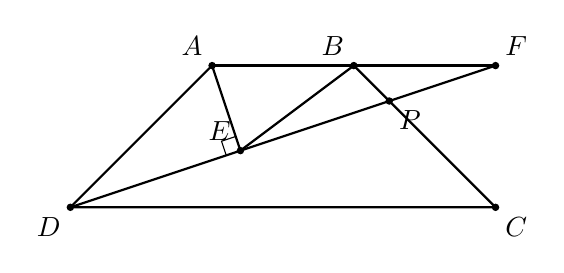
\begin{tikzpicture}[scale=0.9]
\coordinate (D) at (-2,0);
\coordinate (C) at (4,0);
\coordinate (A) at (0,2);
\coordinate (B) at (2,2);
\coordinate (P) at (2.5,1.5);
\coordinate (F) at (4,2);
\coordinate (E) at ($(D)!(A)!(F)$);

\draw[thick] (B) -- (C) -- (D) -- (A);
\draw[thick] (D) -- (F);
\draw[thick] (A) -- (F);
\draw[thick] (A) -- (E);
\draw[thick] (B) -- (E);
\draw ($(E)!6pt!(A)$) -- ($($(E)!6pt!(A)$)+($(E)!6pt!(D)$)-(E)$) -- ($(E)!6pt!(D)$);

\foreach \p in {A,B,C,D,P,F,E} \fill (\p) circle (1.5pt);

\node[above left] at (A) {$A$};
\node[above left] at (B) {$B$};
\node[below right] at (C) {$C$};
\node[below left] at (D) {$D$};
\node[below right] at (P) {$P$};
\node[above right] at (F) {$F$};
\node[above left] at (E) {$E$};
\end{tikzpicture}
\end{center}

Trikampiai $PCD$ ir $PBF$ panašūs: $\angle CPD=\angle BPF$ kaip kryžminiai; $\angle PDC\hm=\angle PFB$, $\angle PCD=\angle PBF$ kaip priešiniai ($AB\parallel CD$). Panašumo koeficientas lygus $\frac{FB}{DC}=\frac{BP}{CP}=\frac{AB}{DC}$. Todėl $FB=AB$.

Nagrinėkime statųjį trikampį $AEF$. Jo įžambinė $AF$ yra jo apibrėžtinio apskritimo skersmuo (į ją remiasi statusis kampas). Skersmens $AF$ vidurio taškas $B$ yra apibrėžtinio apskritimo centras ($AB=BF$), o atkarpos $BA$, $BF$, $BE$ yra šio apskritimo spinduliai. Vadinasi, $AB=BE$.
 \vspace{0,3cm}


\begin{uzdavinys}
Ar lygiakraštį trikampį galima padalyti į 2007 lygiakraščius trikampius?
\end{uzdavinys}

\textit{Pirmasis sprendimas.} Lygiakraščio trikampio vidurio linijos dalija jį į 4 lygiakraščius trikampius. Taip iš vieno trikampio gauname keturis, t.~y.~trikampių padidėja trimis. Jei vieną iš gautųjų trikampių vėl taip pat padalysime į 4 trikampius, tai gausime dar 3 trikampiais daugiau, t.~y.~iš viso $1+3+3=7$ trikampius. Tęsdami šį procesą, gausime $1+3+3+\ldots+3=1+3n$ trikampių, kai $n=1$, 2, 3, $\ldots$. Tačiau trikampių~skai\-čiaus~2007, kuris dalijasi iš 3 be liekanos, negausime. Visgi jį galima gauti kiek~\mbox{kitaip}.

Keturis lygiakraščius~trikam\-pėlius, sudarančius lygiakraštį trikampį, įsivaizduokime sudėtus dviem eilėmis: viršutinėje eilėje vienas, o apatinėje trys trikampėliai. Sudėję dar vieną tokių pačių trikampėlių eilę apačioje, gausime lygiakraštį trikampį, padalytą į $1+3+5=9$ trikampėlius~(žr.~pav.~kairėje).
 
Taigi kiekvieną lygiakraštį trikampį galima padalyti į 9 mažesnius (atkarpomis, kurios lygiagrečios su kraštinėmis ir dalija jas į lygias dalis). Toliau bet kurį jau turimą trikampėlį galima vėl dalyti į 4 arba 9 mažesnius, taip pridedant po 3 ar 8 trikampėlius. Vis dalydami į 4 trikampius, galime gauti $9+3+3+\ldots+3=3n$ trikampėlių, kai $n=3$,~$4$,~$5$,~$\ldots$. Vadinasi, lygiakraštį trikampį galima padalyti ir į $3\cdot669=2007$ lygiakraščius trikampius. 

\vspace{-0mm}
\begin{center}
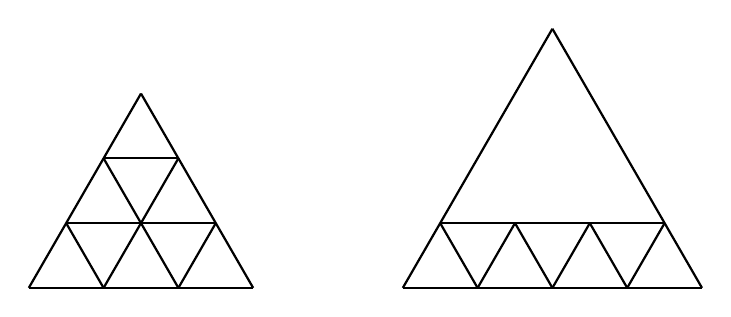
\begin{tikzpicture}[scale=0.95]
% Left figure
\begin{scope}[xshift=0cm]
\draw[thick] (0,0) -- (3,0);
\draw[thick] (0.5, {sqrt(3)/2}) -- (2.5, {sqrt(3)/2});
\draw[thick] (1, {sqrt(3)}) -- (2, {sqrt(3)});
\draw[thick] (0,0) -- (1.5, {1.5*sqrt(3)});
\draw[thick] (1,0) -- (2, {sqrt(3)});
\draw[thick] (2,0) -- (2.5, {sqrt(3)/2});
\draw[thick] (3,0) -- (1.5, {1.5*sqrt(3)});
\draw[thick] (2,0) -- (1, {sqrt(3)});
\draw[thick] (1,0) -- (0.5, {sqrt(3)/2});
\end{scope}

% Right figure
\begin{scope}[xshift=5cm]
\draw[thick] (0,0) -- (4,0);
\draw[thick] (0.5, {sqrt(3)/2}) -- (3.5, {sqrt(3)/2});
\draw[thick] (0,0) -- (2, {2*sqrt(3)});
\draw[thick] (1,0) -- (1.5, {sqrt(3)/2});
\draw[thick] (2,0) -- (2.5, {sqrt(3)/2});
\draw[thick] (3,0) -- (3.5, {sqrt(3)/2});
\draw[thick] (4,0) -- (2, {2*sqrt(3)});
\draw[thick] (3,0) -- (2.5, {sqrt(3)/2});
\draw[thick] (2,0) -- (1.5, {sqrt(3)/2});
\draw[thick] (1,0) -- (0.5, {sqrt(3)/2});
\end{scope}
\end{tikzpicture}
\end{center}
\vspace{-1mm}

\emph{Antrasis sprendimas.} Tegu $n$ yra bet koks natūralusis skaičius, didesnis už 1. Pasirinkime vieną lygiakraščio trikampio kraštinę. Laikykime, kad jos ilgis lygus 1, ir padalykime ją į $n$ lygių atkarpų. Kiekviena iš $n$ atkarpų yra lygiakraščio trikampėlio, kuris yra pradinio trikampio viduje, kraštinė. Gauname $n$ tokių trikampėlių. Tarp kiekvienų dviejų gretimų trikampėlių galima įterpti dar po vieną tokį patį trikampėlį. Taip gauname dar $n-1$ trikampėlį (žr.~pav.~dešinėje, čia $n=4$). Likusi pradinio~tri\-kam\-pio dalis yra lygiakraštis trikampis (jo kraštinių ilgiai yra $1-\frac1n=\frac{n-1}n$, \,$1-\frac1n=\frac{n-1}n$~ir $(n-1)\cdot\frac1n=\frac{n-1}n$).
 Pradinis trikampis padalytas į $n+(n-1)+1=2n$ lygiakraščių trikampių. Vieną iš šių $2n$ trikampių dar padaliję į 4 lygiakraščius trikampius (kaip pirmajame sprendime), pradinį trikampį būsime padaliję į $2n+3$ trikampius. Vadinasi, lygiakraštį trikampį galima padalyti į $2\cdot1002+3=2007$ lygiakraščius trikampius. 


\emph{Pastaba.} Iš šio sprendimo išplaukia, kad lygiakraštį trikampį galima padalyti į $2n$ ir į $2n+3$ lygiakraščius trikampius, kai $n=2$, 3, 4, $\ldots$, taigi į $m$ tokių trikampių, kur $m=6$, 7, 8, $\ldots$. Taip pat tinka $m=4$. Tuo tarpu į du, tris arba penkis lygiakraščius trikampius lygiakraščio trikampio padalyti nepavyks. 

\begin{flushright}
Ats.: taip, galima.
\end{flushright}
 \vspace{0,7cm}


\end{document}